% -*- latex -*-
%%%%%%%%%%%%%%%%%%%%%%%%%%%%%%%%%%%%%%%%%%%%%%%%%%%%%%%%%%%%%%%%
%%%%%%%%%%%%%%%%%%%%%%%%%%%%%%%%%%%%%%%%%%%%%%%%%%%%%%%%%%%%%%%%
%%%%
%%%% This text file is part of the source of 
%%%% `Parallel Computing'
%%%% by Victor Eijkhout, copyright 2012-9
%%%%
%%%% pearc19-advanced.tex : introduction to Advanced MPI at PEARC19
%%%%
%%%%%%%%%%%%%%%%%%%%%%%%%%%%%%%%%%%%%%%%%%%%%%%%%%%%%%%%%%%%%%%%
%%%%%%%%%%%%%%%%%%%%%%%%%%%%%%%%%%%%%%%%%%%%%%%%%%%%%%%%%%%%%%%%

\documentclass[11pt,headernav]{beamer}

\beamertemplatenavigationsymbolsempty
\usetheme{Madrid}%{Montpellier}
\usecolortheme{seahorse}
\setcounter{tocdepth}{1}
\AtBeginSection[]
{
  \begin{frame}
    \frametitle{In this section}
    \tableofcontents[currentsection]
  \end{frame}
}
%% \AtBeginPart
%% {
%%   \begin{frame}
%%     \frametitle{Table of Contents}
%%     \tableofcontents
%%   \end{frame}
%% }

\setbeamertemplate{footline}{\hskip1em Eijkhout: Advanced MPI\hfill
  \hbox to 0in {\hss 
\includegraphics[scale=.1]{tacclogonew}}%
  \hbox to 0in {\hss \arabic{page}\hskip 1in}}

\usepackage{multicol,multirow}
% custom arrays and tables
\usepackage{array} %,multirow,multicol}
\newcolumntype{R}{>{\hbox to 1.2em\bgroup\hss}{r}<{\egroup}}
\newcolumntype{T}{>{\hbox to 8em\bgroup}{c}<{\hss\egroup}}

\input acromacs
\input slidemacs
\input coursemacs
\input listingmacs

\def\Location{}% redefine in the inex file
\input inex
\def\Location{PEARC 2019 tutorial}

%%%%%%%%%%%%%%%%
%%%%%%%%%%%%%%%% Document
%%%%%%%%%%%%%%%%

\begin{document}
\parskip=10pt plus 5pt minus 3pt

\title{An Introduction to Advanced Features of MPI}
\author{Victor Eijkhout {\tt eijkhout@tacc.utexas.edu}}
\date{\Location}

\begin{frame}
  \titlepage
\end{frame}

\begin{frame}\frametitle{Code of Conduct}
  \scriptsize
  XSEDE has an external code of conduct for XSEDE sponsored events
  which represents XSEDE's commitment to providing an inclusive and
  harassment-free environment in all interactions regardless of
  gender, sexual orientation, disability, physical appearance, race,
  or religion. The code of conduct extends to all XSEDE-sponsored
  events, services, and interactions.

  Code of Conduct: \url{https://www.xsede.org/codeofconduct}

  Contact:
  \begin{itemize}
  \item Teacher: Victor Eijkhout \texttt{eijkhout@tacc.utexas.edu}\\
  \item  Event organizer: Jason Allison  \texttt{jasona@tacc.utexas.edu}
  \end{itemize}
  XSEDE ombudspersons:
  \begin{itemize}
  \item
    Linda Akli, Southeastern Universities Research Association
    \texttt{akli@sura.org}
  \item 
    Lizanne Destefano, Georgia Tech
    \texttt{lizanne.destefano@ceismc.gatech.edu}
  \item 
    Ken Hackworth, Pittsburgh Supercomputing Center \texttt{hackworth@psc.edu}
  \item 
    Bryan Snead, Texas Advanced Computing Center
    \texttt{jbsnead@tacc.utexas.edu}
  \end{itemize}
\end{frame}

\begin{frame}{Justification}
  MPI-3 adds a number of features to MPI that offer more elegant
  expression of algorithms, or higher performance.
\end{frame}

\begin{frame}[containsverbatim]\frametitle{Note on the exercises}
  \begin{itemize}
  \item Get the exercises on stampede2 from
    \n{~train00/advanced-mpi.tgz} or \n{URL} and unpack.
  \item Most exercises are available in C, C++, F90, F2008, and Python.
  \item Exercise slides have the name of the file in the header.
  \item Each exercise file has clearly indicated what information you
    need to supply.
  \item There is a makefile for compiling and testing the exercises.
  \end{itemize}
\end{frame}

\Level 0 {This should have been in MPI-1}

\sectionframe{Subarray type}

\begin{frame}[containsverbatim]{Reminder: vector type}
  \mpiRoutineRef{MPI_Type_vector}
\end{frame}

\begin{frame}[containsverbatim]\frametitle{Submatrix storage 2D}
  Three parameter BLAS/Lapack description:

  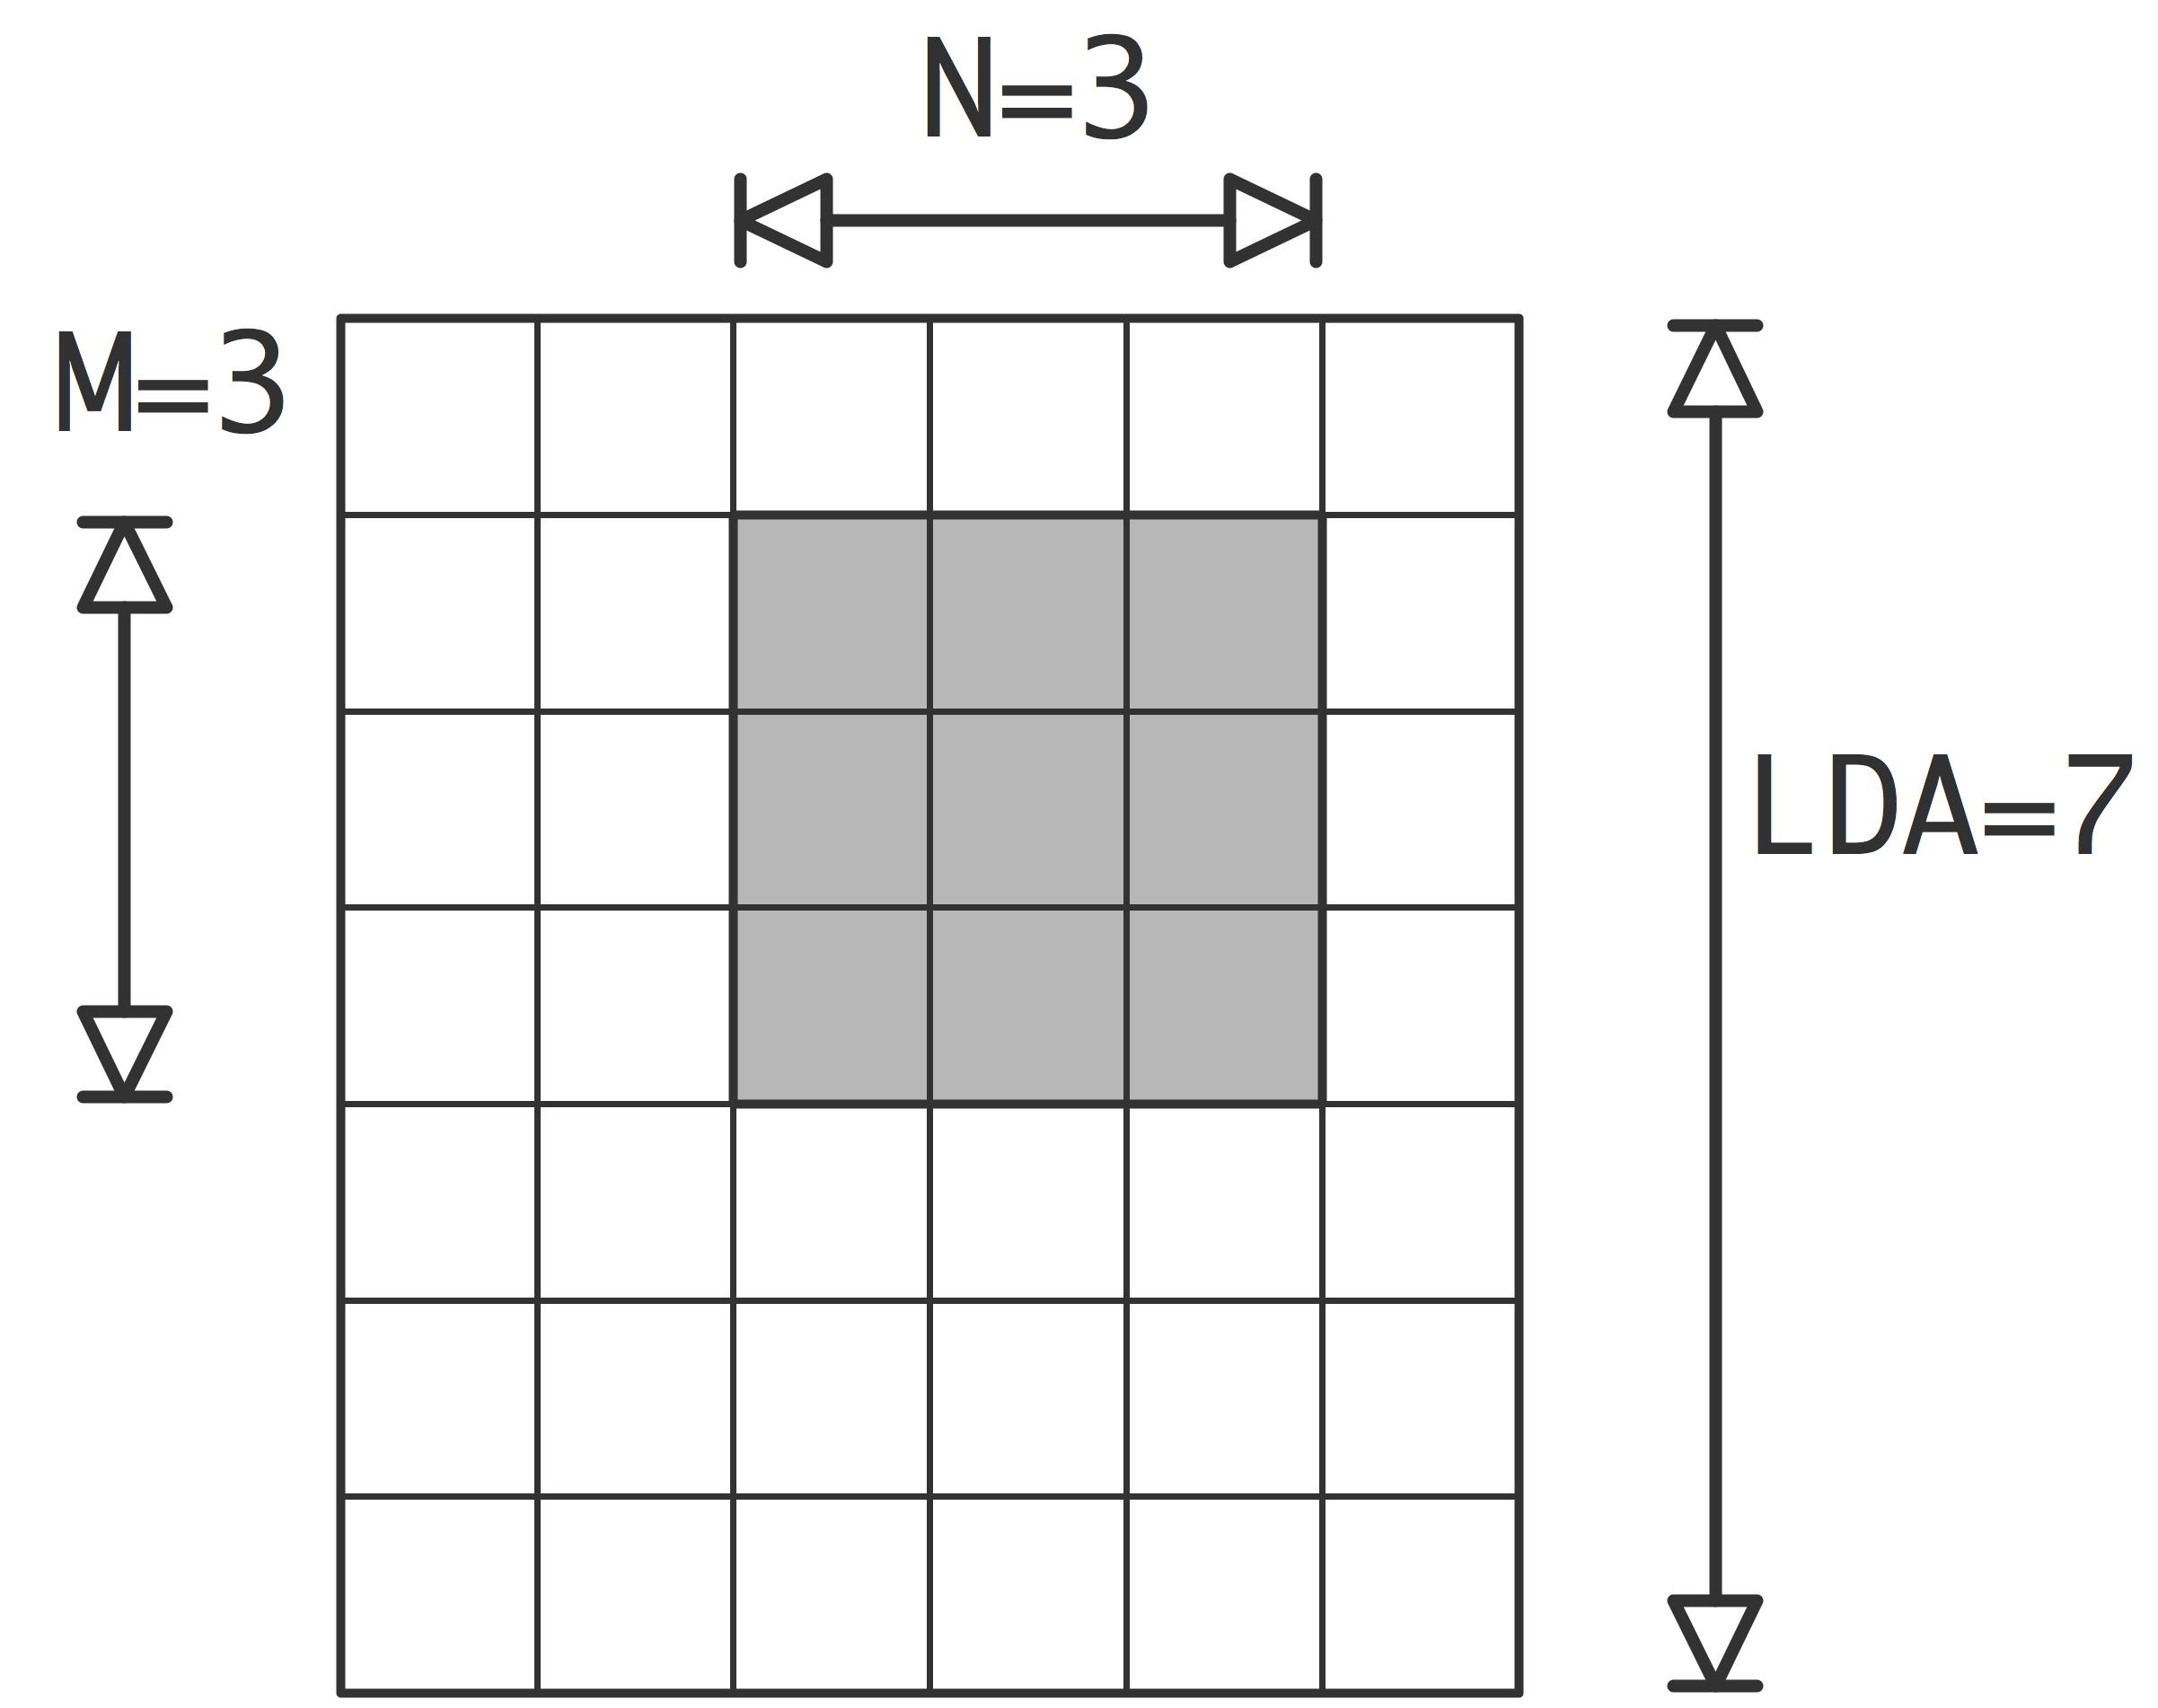
\includegraphics[scale=.06]{blasmatrix}  

  Vector type:\\
  Blocksize: M,  Stride: LDA, Number of blocks: N
\end{frame}

\begin{frame}[containsverbatim]\frametitle{Subarray type}
  \begin{itemize}
  \item Vector type is convenient for 2D subarrays,
  \item it gets tedious for subarrays in higher dimensions.
  \item Better solution: \indexmpishow{MPI_Type_create_subarray}
  \item Description of
    \begin{itemize}
    \item Outer brick size
    \item Inner brick size
    \item Location of `top left corner of inner brick
    \end{itemize}
  \end{itemize}
\end{frame}

\begin{frame}[containsverbatim]\frametitle{Subarray type}
  \mpiRoutineRef{MPI_Type_create_subarray}
\end{frame}

\begin{exerciseframe}[cubegather]
  \input ex:cubegather
\end{exerciseframe}

\Level 0 {One-sided communication}
\input Onesided-slides 

\Level 0 {Shared memory}
\input Sharedmemory-slides

\Level 0 {Advanced collectives}
\input Highercollective-slides

\Level 0 {Process management}
\input Spawn-slides

\Level 0 {Process topologies}
\input Graph-slides

\Level 0 {Beginner exercise}

\begin{exerciseframe}
  \input ex:serialsend
\end{exerciseframe}

\end{document}

